\documentclass[conference]{IEEEtran}
\IEEEoverridecommandlockouts

\usepackage{cite}
\usepackage{amsmath,amssymb,amsfonts}
\usepackage{graphicx}
\usepackage{textcomp}
\usepackage{xcolor}
\usepackage{booktabs}
\usepackage{array}
\usepackage{tikz}
\usetikzlibrary{shapes.geometric, arrows.meta, positioning}
\usepackage[hidelinks]{hyperref}

\graphicspath{{figures/}}

\begin{document}

\title{Explainable Multi-Class Thyroid-Disease Classification from\\
Laboratory Panels: A Detailed Study of Tree-Ensemble Models,\\
Their Training, and Per-Prediction SHAP Interpretation}

\author{
\IEEEauthorblockN{Aditya Dhull}
\IEEEauthorblockA{\textit{Independent Study in Applied Machine Learning} \\
\texttt{adityadhull@iisc.ac.in}}
}

\maketitle

\begin{abstract}
Thyroid dysfunction is among the most common endocrine disorders, and its
diagnosis rests almost entirely on a small panel of laboratory measurements
governed by a well-understood feedback loop. This makes it an ideal testbed for
machine-learning models that must be both accurate and \emph{explainable}. We
present a detailed, reproducible framework that classifies patients into seven
clinically coherent thyroid categories from the Garavan Institute archive
($n{=}9{,}172$), a large, severely imbalanced ($73.8\%$ majority) dataset with
informative missing laboratory values. We study five tree-ensemble models in
depth---Random Forest, XGBoost, a soft-voting hybrid of the two, LightGBM, and a
stacking ensemble---explaining the learning principle, the optimisation
objective, and the exact training procedure of each. We describe a leakage-safe
preprocessing and cross-validation methodology, an explicit treatment of class
imbalance, and a statistical protocol for comparing models. The hybrid attains a
hold-out accuracy of $0.945$ and macro-F1 of $0.863$, with a paired $t$-test
confirming a statistically significant improvement over the Random-Forest baseline
($p{=}0.014$). We then use exact TreeSHAP to produce both global feature
attributions and \emph{detailed per-prediction} explanations that recover textbook
thyroid physiology (e.g.\ suppressed TSH with elevated free-thyroxine index
driving a hyperthyroid prediction). The result is a transparent pipeline whose
every decision can be audited against clinical reasoning.
\end{abstract}

\begin{IEEEkeywords}
Thyroid disease, Random Forest, XGBoost, LightGBM, stacking, soft voting, SHAP,
explainable AI, class imbalance, gradient boosting.
\end{IEEEkeywords}

\section{Introduction}
The thyroid gland regulates basal metabolic rate through the hormones thyroxine
(T4) and triiodothyronine (T3), whose secretion is controlled by pituitary
thyroid-stimulating hormone (TSH) under negative feedback. Because a handful of
serum measurements (TSH, T3, total T4, thyroxine-binding capacity, and the free
thyroxine index) capture this axis almost completely, thyroid status is a problem
where a machine-learning model's reasoning can be checked directly against
physiology. This is rarely true in clinical ML, and it is the central motivation
for this study.

We address a seven-class formulation that distinguishes the normal state from
hypothyroidism, hyperthyroidism, binding-protein anomalies, non-thyroidal illness,
ongoing replacement therapy, and discordant assay results. The dataset is large
($9{,}172$ patients), heavily imbalanced, and contains laboratory values that are
\emph{missing not at random}---a panel is ordered when a clinician suspects a
problem, so the absence of a measurement is itself informative. These properties
make the problem a realistic stress test rather than a sanitised benchmark.

This paper emphasises \emph{depth} on two fronts that are often compressed in
applied studies: (i) a careful account of every model and exactly how it is
trained, and (ii) per-prediction explanations. Our contributions are a detailed
comparative treatment of five tree ensembles and their training methodology; a
leakage-safe, imbalance-aware evaluation protocol; a statistically grounded model
comparison; and exact SHAP explanations at both the global and the individual-
patient level.

\section{Clinical Background}
\subsection{The Hypothalamic--Pituitary--Thyroid Axis}
The hypothalamus secretes thyrotropin-releasing hormone, prompting the pituitary
to release TSH, which stimulates the thyroid to produce T4 and T3. Circulating
thyroid hormone then suppresses further TSH release---a thermostat. When the
\emph{gland} fails, hormone falls and TSH rises to compensate; when the gland is
overactive, hormone rises and TSH is suppressed. TSH and thyroid hormone therefore
move in \emph{opposite} directions in primary disease, and because TSH responds
logarithmically it is the single most sensitive screening test. A model trained on
these features should, and does, lean heavily on TSH.

\subsection{The Seven Target Classes}
We group the archive's raw diagnosis codes into: \textit{negative} (no thyroid
condition), \textit{hypothyroid} (under-active; high TSH, low free T4),
\textit{hyperthyroid} (over-active; suppressed TSH, high T4/T3),
\textit{binding\_protein} (altered thyroxine-binding globulin, e.g.\ from
pregnancy or estrogen, shifting \emph{total} but not free hormone),
\textit{nonthyroidal\_illness} (the ``sick-euthyroid'' pattern, typically low T3
in seriously ill patients), \textit{replacement\_therapy} (patients on exogenous
thyroxine), and \textit{discordant\_results} (assays that disagree). Several of
these classes are physiologically subtle, which is why a clean test of an
explainable model is valuable.

\section{Dataset and Preprocessing}
\subsection{Data}
The Garavan \texttt{thyroid0387} archive contains $9{,}172$ records with $29$
attributes and a diagnosis string. Six attributes are continuous laboratory
values (age, TSH, T3, total~T4, T4U, FTI); fourteen are binary clinical-history
flags (e.g.\ \textit{on\_thyroxine}, \textit{pregnant}, \textit{lithium},
\textit{thyroid\_surgery}); two are nominal (sex, referral source). The class
distribution (Fig.~\ref{fig:dist}) is dominated by the negative class
($73.8\%$), with the rarest disease class (hyperthyroid) at $2.9\%$.

\subsection{Cleaning, Encoding and Missingness}
We map the diagnosis codes to the seven groups above, taking the more-likely label
where the archive records an ambiguous ``X$\mid$Y'' code, and folding the small
antithyroid-treatment codes into the hyperthyroid group (they denote hyperthyroid
management). Binary flags are mapped $\{f,t\}\!\to\!\{0,1\}$; a non-physiological
age ${>}120$ is treated as missing; the near-empty TBG measurement and the
redundant ``measured'' indicator columns are dropped.

Crucially, several laboratory values are missing for a large fraction of patients
(T3 in $28\%$, TSH in $9\%$). Rather than discard these rows, we
\emph{median-impute} each numeric feature and append a binary
\emph{missing-indicator} column so the model can learn from the fact that a test
was not ordered. Nominal features are most-frequent imputed and one-hot encoded.
Because tree ensembles are invariant to monotone feature scaling, no
standardisation is applied. The complete transform is encapsulated in a
\texttt{ColumnTransformer} that is fit only on training data (Section~\ref{sec:leak}).

\begin{figure}[t]
\centering

\includegraphics[width=0.95\columnwidth]{thyroid_class_dist.png}
\caption{Class distribution of the seven thyroid groups. The problem is severely
imbalanced, motivating macro-averaged metrics and imbalance-aware training.}
\label{fig:dist}
\end{figure}

\section{Models}
All five models are tree-based, a deliberate choice: trees handle mixed feature
types and missing-indicator flags natively, require no scaling, capture the
threshold logic of clinical decision-making (``TSH${>}6$ \emph{and}
FTI${<}60$''), and admit \emph{exact} SHAP explanations. We now describe each
model, its learning principle, and its training.

\subsection{Foundation: the Decision Tree}
A decision tree partitions feature space by recursively choosing the
feature/threshold that most reduces node impurity, measured for a node with class
proportions $p_c$ by the Gini index $G=1-\sum_c p_c^2$ or entropy
$H=-\sum_c p_c\log p_c$. A leaf predicts the empirical class distribution of its
training samples. A single deep tree has low bias but high variance: it
memorises the training set. The two ensemble families below tame this variance and
bias in complementary ways, which is exactly why combining them is attractive.

\subsection{Random Forest (Bagging)}
A Random Forest averages $T$ decorrelated trees,
\begin{equation}
f_{\mathrm{RF}}(x)=\frac{1}{T}\sum_{t=1}^{T}h_t(x),
\end{equation}
where each $h_t$ is grown on a \emph{bootstrap} resample of the training data
(rows drawn with replacement) and, at every split, considers only a random subset
of features (typically $\sqrt{d}$). These two randomisations decorrelate the
trees. If individual trees have variance $\sigma^2$ and pairwise correlation
$\rho$, the average has variance
\begin{equation}
\rho\,\sigma^2+\frac{1-\rho}{T}\,\sigma^2,
\end{equation}
so lowering $\rho$ (via the randomisation) and increasing $T$ both reduce variance
without raising bias---the essence of \emph{bagging}. For multi-class problems each
tree outputs a class distribution and the forest averages them, giving calibrated
\texttt{predict\_proba} outputs that the hybrid later consumes. We use $T{=}300$
fully grown trees. Imbalance is handled with \texttt{class\_weight} =
\texttt{balanced\_subsample}, which reweights classes within each bootstrap
(Section~\ref{sec:imb}).

\subsection{XGBoost (Gradient Boosting)}
Where bagging reduces variance, \emph{boosting} reduces bias by building trees
\emph{sequentially}, each correcting its predecessors. XGBoost fits an additive
model $\hat{y}_i^{(t)}=\hat{y}_i^{(t-1)}+f_t(x_i)$ by minimising, at step $t$, the
regularised objective
\begin{equation}
\mathcal{L}^{(t)}=\sum_{i=1}^{N}\ell\!\left(y_i,\hat{y}_i^{(t-1)}+f_t(x_i)\right)
+\Omega(f_t),
\end{equation}
with complexity penalty $\Omega(f)=\gamma T+\tfrac{1}{2}\lambda\sum_j w_j^2$ over a
tree's $T$ leaves and leaf weights $w_j$. Expanding the loss to second order with
gradients $g_i=\partial_{\hat{y}}\ell$ and Hessians $h_i=\partial^2_{\hat{y}}\ell$
gives the per-leaf optimum and the resulting structure score
\begin{equation}
w_j^\star=-\frac{G_j}{H_j+\lambda},\qquad
\tilde{\mathcal{L}}=-\frac{1}{2}\sum_{j}\frac{G_j^2}{H_j+\lambda}+\gamma T,
\end{equation}
where $G_j=\sum_{i\in I_j}g_i$ and $H_j=\sum_{i\in I_j}h_i$ aggregate over the
samples in leaf $j$. A candidate split is scored by the gain
\begin{equation}
\mathrm{Gain}=\tfrac{1}{2}\!\left[\frac{G_L^2}{H_L+\lambda}+\frac{G_R^2}{H_R+\lambda}
-\frac{(G_L+G_R)^2}{H_L+H_R+\lambda}\right]-\gamma,
\end{equation}
and accepted only if positive---this is how $\lambda$ and $\gamma$ prevent
overfitting at the level of individual splits. We use the multi-class softmax
objective (\texttt{multi:softprob}), $400$ trees of depth $6$, a learning rate
(shrinkage) of $0.1$ that scales each tree's contribution, row and column
subsampling of $0.9$ (borrowing bagging's decorrelation), $\lambda{=}1$, and the
fast histogram split-finder. Because XGBoost has no \texttt{class\_weight}, we pass
\emph{balanced per-sample weights} (Section~\ref{sec:imb}).

\subsection{The Hybrid: Soft Voting}
The hybrid combines the variance-reducing forest and the bias-reducing booster by
averaging their posterior probabilities and taking the arg-max,
\begin{equation}
\hat{y}=\arg\max_{c\in\{1,\dots,K\}}\frac{1}{M}\sum_{m=1}^{M}P_m(c\mid x),
\qquad M=2.
\label{eq:soft}
\end{equation}
This is \emph{soft} voting: it uses each model's confidence, so a decisive model
sways the average more than a hesitant one. The two learners' errors are partly
uncorrelated, so the average cancels some of each. Both base learners sit behind a
single shared preprocessing transform, guaranteeing identical inputs.

\subsection{LightGBM}
LightGBM is a second gradient booster with two efficiency innovations.
\emph{Leaf-wise} (best-first) growth splits the leaf with the largest loss
reduction rather than expanding a whole level, producing deeper, more accurate
trees for the same leaf budget. \emph{Histogram} binning buckets continuous
features to accelerate split finding. It further uses gradient-based one-side
sampling (keeping large-gradient samples while sub-sampling small-gradient ones)
and exclusive-feature bundling (merging sparse, mutually-exclusive features). We
use $400$ trees, $63$ leaves, and a learning rate of $0.05$, with
\texttt{class\_weight} = \texttt{balanced}.

\subsection{Stacking}
Soft voting combines models with \emph{fixed equal} weights. Stacking instead
\emph{learns} the combination. Level-0 base learners (Random Forest, XGBoost,
LightGBM) are trained, and their \emph{out-of-fold} predicted probabilities---
obtained by internal $5$-fold cross-validation so the meta-features are
leakage-free---become the inputs to a level-1 meta-learner, here a multinomial
logistic regression with balanced class weights. The meta-learner can discover,
for example, that XGBoost is more trustworthy for one class while the forest is
better for another, an adaptivity that fixed-weight voting cannot express. The
cost is more computation and a greater risk of overfitting, which we limit by
keeping the meta-learner linear.

\section{Training Methodology}
\subsection{Leakage-Safe Pipeline}
\label{sec:leak}
Every model is a scikit-learn \texttt{Pipeline} whose first stage is the
preprocessing \texttt{ColumnTransformer} and whose second stage is the classifier.
When the pipeline is fit, imputation medians and one-hot vocabularies are learned
from the \emph{training partition only}; at validation/test time these learned
transforms are merely applied. Because cross-validation clones and re-fits the
entire pipeline on each fold, no statistic computed on a held-out fold can leak
into training---a frequent and silent source of over-optimistic results that this
design eliminates by construction (Fig.~\ref{fig:arch}).

\subsection{Stratified Splitting and Cross-Validation}
We hold out $20\%$ of patients as a test set with \emph{stratified} sampling,
which preserves each class's proportion; on a problem where the rarest class is
$2.9\%$ of data, a naive split could leave that class with too few test cases to
estimate recall. On the remaining $80\%$ we run stratified five-fold
cross-validation, training each model five times and reporting the mean and
standard deviation of each metric, with the fold standard deviation
\begin{equation}
\sigma=\sqrt{\tfrac{1}{4}\sum_{j=1}^{5}\left(S_j-\mu\right)^2}.
\end{equation}
We retain the \emph{individual} fold scores because the significance test
(Section~\ref{sec:stats}) compares two models fold-by-fold on identical splits.

\subsection{Class-Imbalance Handling}
\label{sec:imb}
With a $73.8\%$ majority, a model can score high accuracy while ignoring every
disease. We counter this in two equivalent ways. For Random Forest, LightGBM and
the stacking meta-learner we set balanced class weights
\begin{equation}
w_c=\frac{N}{K\,n_c},
\end{equation}
which up-weights a class inversely to its frequency $n_c$. XGBoost, lacking a
class-weight argument, receives the same correction as \emph{per-sample} weights
$w_i=w_{y_i}$ at fit time. (Synthetic minority over-sampling, applied inside the
training fold, is supported as an alternative.) Coupled with macro-averaged
metrics, this ensures rare diseases materially affect both training and scoring.

\subsection{Hyperparameter Configuration}
Table~\ref{tab:hp} lists the configuration of every model. These are strong,
lightly-tuned defaults chosen for a fair comparison rather than exhaustively
optimised; all share a fixed random seed ($42$) for reproducibility.

\begin{table}[t]
\caption{Model hyperparameters.}
\label{tab:hp}
\centering
\footnotesize
\renewcommand{\arraystretch}{1.2}
\begin{tabular}{p{1.7cm}p{6cm}}
\toprule
\textbf{Model} & \textbf{Key settings} \\
\midrule
Random Forest & $300$ trees, unlimited depth, $\sqrt{d}$ features/split,
\texttt{balanced\_subsample} weights \\
XGBoost & $400$ trees, depth $6$, lr $0.1$, subsample $0.9$, colsample $0.9$,
$\lambda{=}1$, \texttt{multi:softprob}, hist, balanced sample weights \\
LightGBM & $400$ trees, $63$ leaves, lr $0.05$, subsample $0.9$, colsample $0.9$,
\texttt{balanced} weights \\
Hybrid & soft voting of the above RF and XGBoost ($M{=}2$, equal weights) \\
Stacking & base: RF, XGBoost, LightGBM; meta: multinomial logistic regression
($5$-fold out-of-fold features) \\
\bottomrule
\end{tabular}
\end{table}

\subsection{Environment and Reproducibility}
Experiments use Python with scikit-learn, XGBoost, LightGBM and the SHAP library.
All randomness (splits, bootstraps, column sampling, fold shuffling) is seeded;
the data download, preprocessing, training, evaluation and figure generation run
from a single scripted pipeline so the entire study is reproducible end-to-end.

\begin{figure}[t]
\centering
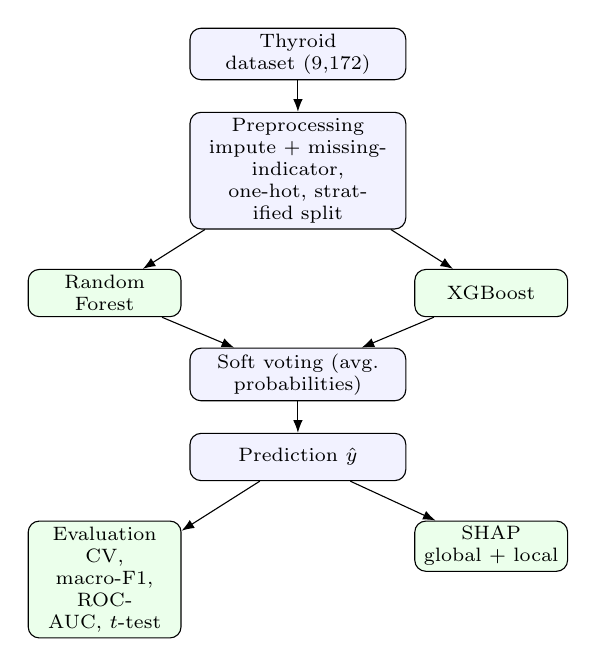
\begin{tikzpicture}[
  node distance=4mm and 6mm,
  box/.style={draw, rounded corners, align=center, font=\scriptsize,
              minimum height=6mm, inner sep=2pt, fill=blue!5, text width=26mm},
  base/.style={draw, rounded corners, align=center, font=\scriptsize,
              minimum height=6mm, inner sep=2pt, fill=green!8, text width=18mm},
  arr/.style={-{Latex[length=1.6mm]}}]
\node[box] (data) {Thyroid dataset (9{,}172)};
\node[box, below=of data] (prep) {Preprocessing\\impute $+$ missing-indicator,\\one-hot, stratified split};
\node[base, below left=5mm and 1mm of prep] (rf) {Random Forest};
\node[base, below right=5mm and 1mm of prep] (xgb) {XGBoost};
\node[box, below=15mm of prep] (vote) {Soft voting (avg.\ probabilities)};
\node[box, below=of vote] (pred) {Prediction $\hat{y}$};
\node[base, below left=5mm and 1mm of pred] (eval) {Evaluation\\CV, macro-F1,\\ROC-AUC, $t$-test};
\node[base, below right=5mm and 1mm of pred] (shap) {SHAP\\global $+$ local};
\draw[arr] (data) -- (prep);
\draw[arr] (prep) -- (rf);
\draw[arr] (prep) -- (xgb);
\draw[arr] (rf) -- (vote);
\draw[arr] (xgb) -- (vote);
\draw[arr] (vote) -- (pred);
\draw[arr] (pred) -- (eval);
\draw[arr] (pred) -- (shap);
\end{tikzpicture}
\caption{Leakage-safe training and evaluation pipeline. Preprocessing is fit
inside each cross-validation fold.}
\label{fig:arch}
\end{figure}

\section{Evaluation Protocol}
\label{sec:stats}
On a heavily imbalanced problem, plain accuracy is misleading---predicting the
majority class for everyone already scores $0.738$. We therefore foreground
\emph{macro}-averaged F1, which computes F1 per class and averages classes
equally:
\begin{equation}
\mathrm{F1}_i=\frac{2\,\mathrm{Prec}_i\,\mathrm{Rec}_i}{\mathrm{Prec}_i+\mathrm{Rec}_i},
\qquad \mathrm{Macro\text{-}F1}=\frac{1}{K}\sum_{i=1}^{K}\mathrm{F1}_i.
\end{equation}
We also report balanced accuracy (mean per-class recall) and one-vs-rest
ROC--AUC, which uses predicted probabilities and so measures class separation
independent of any threshold. To test whether the hybrid genuinely beats the
Random-Forest baseline we apply a \emph{paired} $t$-test to the fold-wise macro-F1
scores,
\begin{equation}
t=\frac{\bar{d}}{s_d/\sqrt{n}},\qquad n=5,
\end{equation}
where $d_i$ is the per-fold difference. Pairing on identical folds removes
fold-to-fold variance and makes the test sensitive to the model difference itself.

\section{Results}
\subsection{Cross-Validation and Model Comparison}
Table~\ref{tab:cv} reports five-fold cross-validation for all five models, and
Fig.~\ref{fig:cmp} visualises their macro-F1. The hybrid attains the best mean
macro-F1 ($0.875$) with the smallest variance among the classic trio, echoing the
expectation that soft voting improves \emph{stability}. The two boosters (XGBoost,
LightGBM) and stacking are close behind; the gain over plain XGBoost is small, so
most of the lift over the forest comes from boosting rather than from voting
\emph{per se}.

\begin{table}[t]
\caption{Stratified five-fold cross-validation, mean\,$\pm$\,std.}
\label{tab:cv}
\centering
\renewcommand{\arraystretch}{1.2}
\begin{tabular}{lccc}
\toprule
\textbf{Model} & \textbf{Accuracy} & \textbf{Macro-F1} & \textbf{ROC-AUC} \\
\midrule
Random Forest     & $0.941\pm0.008$ & $0.850\pm0.024$ & $0.992$ \\
XGBoost           & $0.950\pm0.006$ & $0.872\pm0.020$ & $0.995$ \\
Hybrid (RF$+$XGB) & $\mathbf{0.952\pm0.005}$ & $\mathbf{0.875\pm0.018}$ & $0.995$ \\
LightGBM          & $0.951\pm0.005$ & $0.873\pm0.018$ & $0.994$ \\
Stacking          & $0.951\pm0.005$ & $0.874\pm0.015$ & $0.991$ \\
\bottomrule
\end{tabular}
\end{table}

\begin{figure}[t]
\centering

\includegraphics[width=0.92\columnwidth]{thyroid_model_cmp.png}
\caption{Mean cross-validated macro-F1 by model.}
\label{fig:cmp}
\end{figure}

\subsection{Statistical Significance}
The paired $t$-test of hybrid versus Random Forest gives $\bar{d}{=}{+}0.0255$,
$t{=}4.16$, $p{=}0.014$: the improvement \emph{is} statistically significant at the
$0.05$ level. The large sample size ($9{,}172$ patients, hence ample fold data)
supplies the statistical power needed to resolve a genuine-but-modest effect---a
contrast with smaller studies where the same kind of improvement is undetectable.

\subsection{Hold-Out Test Performance}
On the unseen $20\%$ test set the hybrid attains accuracy $0.945$, balanced
accuracy $0.850$, macro-F1 $0.863$, weighted-F1 $0.944$ and ROC--AUC $0.995$. The
gap between accuracy and macro-F1 is the imbalance signature: excellent on large
classes, merely good on rare ones. Per-class results (Table~\ref{tab:pc}) show
near-perfect hypothyroid detection (F1~$0.967$), the unambiguous high-TSH signal
being easy to learn, and the weakest performance on the
intrinsically ambiguous discordant-results class (F1~$0.633$)---a class defined by
disagreeing assays where, by construction, no clean signal exists. The confusion
matrices (Figs.~\ref{fig:cm},~\ref{fig:cmn}) and ROC curves
(Fig.~\ref{fig:roc}) confirm strong, well-separated performance across classes.

\begin{table}[t]
\caption{Per-class hold-out performance of the hybrid.}
\label{tab:pc}
\centering
\renewcommand{\arraystretch}{1.2}
\begin{tabular}{lcccc}
\toprule
\textbf{Class} & \textbf{Prec.} & \textbf{Rec.} & \textbf{F1} & \textbf{Support} \\
\midrule
negative              & 0.963 & 0.974 & 0.969 & 1355 \\
hypothyroid           & 0.949 & 0.985 & 0.967 & 132 \\
nonthyroidal illness  & 0.977 & 0.923 & 0.949 & 91 \\
binding protein       & 0.829 & 0.808 & 0.818 & 78 \\
replacement therapy   & 0.903 & 0.915 & 0.909 & 71 \\
discordant results    & 0.738 & 0.554 & 0.633 & 56 \\
hyperthyroid          & 0.804 & 0.789 & 0.796 & 52 \\
\midrule
macro avg             & 0.880 & 0.850 & 0.863 & 1835 \\
\bottomrule
\end{tabular}
\end{table}

\begin{figure}[t]
\centering

\includegraphics[width=0.95\columnwidth]{thyroid_cm.png}
\caption{Confusion matrix of the hybrid on the thyroid hold-out set (counts).}
\label{fig:cm}
\end{figure}

\begin{figure}[t]
\centering

\includegraphics[width=0.95\columnwidth]{thyroid_cm_norm.png}
\caption{Row-normalised confusion matrix (per-class recall on the diagonal).}
\label{fig:cmn}
\end{figure}

\begin{figure}[t]
\centering

\includegraphics[width=0.92\columnwidth]{thyroid_roc.png}
\caption{One-vs-rest ROC curves per class for the hybrid.}
\label{fig:roc}
\end{figure}

\section{Explainability}
\subsection{Global Attribution}
For a tree model and target class, SHAP decomposes a prediction additively,
$f(x)=\phi_0+\sum_j\phi_j$, with base value $\phi_0$ and signed per-feature
contributions $\phi_j$ computed exactly by TreeSHAP. Averaging $|\phi_j|$ over all
patients yields the global importances in Fig.~\ref{fig:shapbar}: TSH, T3, FTI,
total~T4, \textit{on\_thyroxine} and T4U lead, exactly the thyroid function panel
in clinically sensible order. The SHAP \emph{interaction} summary
(Fig.~\ref{fig:bee}) decomposes each contribution into a main effect (the matrix
diagonal) and pairwise interaction effects (off-diagonal cells): the dominant cells
involve TSH, total~T4 and FTI, and the TSH$\times$FTI and TSH$\times$TT4
interactions encode the clinical rule that TSH must be interpreted \emph{together}
with a thyroid-hormone level rather than alone. The high rank of the T3 and TSH
missing-indicators confirms that \emph{which} tests were ordered is itself
diagnostic.

\begin{figure}[t]
\centering
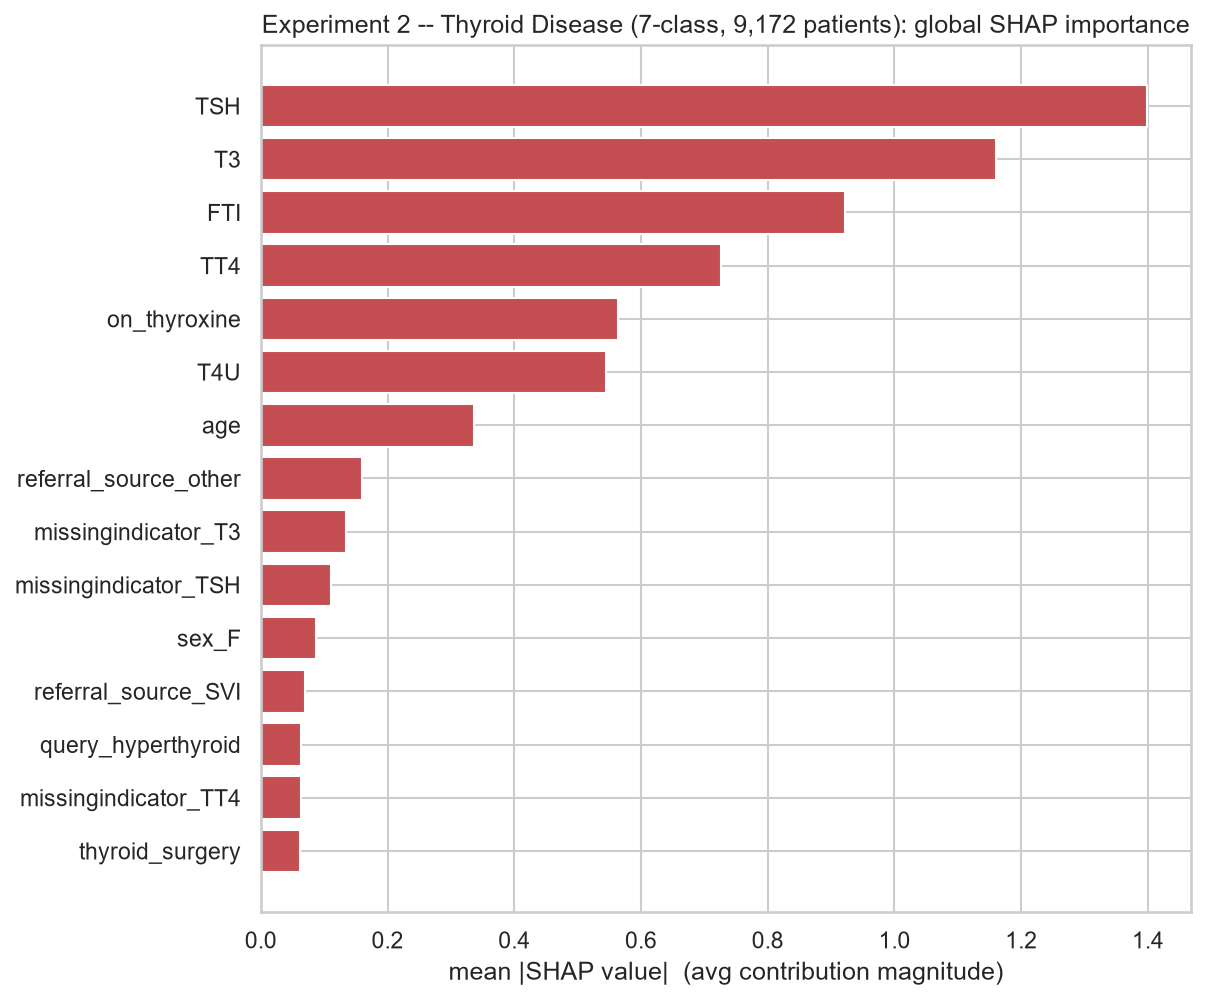
\includegraphics[width=0.95\columnwidth]{thyroid_shap_bar.png}
\caption{Global SHAP importance (mean $|\phi_j|$) of the XGBoost component.}
\label{fig:shapbar}
\end{figure}

\begin{figure*}[t]
\centering

\includegraphics[width=0.82\textwidth]{thyroid_shap_interaction.png}
\caption{SHAP interaction-value summary for the hypothyroid output. The top seven
features appear on both axes; each cell is a beeswarm of SHAP \emph{interaction}
values (x-axis), with colour encoding the feature value. Diagonal cells are a
feature's main effect; off-diagonal cells are pairwise interactions.}
\label{fig:bee}
\end{figure*}

\subsection{Per-Prediction Explanations}
The additive decomposition lets us narrate individual predictions. Three
representative correctly-classified patients:
\begin{itemize}
\item \textbf{Hyperthyroid} (Fig.~\ref{fig:wf_hyper}): a very high free-thyroxine
index (FTI${=}196$, ${+}3.21$) and a suppressed TSH ($0.02$, ${+}2.21$) dominate---
the textbook over-active-gland signature.
\item \textbf{Hypothyroid} (Fig.~\ref{fig:wf_hypo}): an elevated TSH ($6.4$,
${+}3.80$) overwhelmingly drives the prediction, as the feedback loop predicts.
\item \textbf{Replacement therapy} (Fig.~\ref{fig:wf_rep}): the
\textit{on\_thyroxine} flag (${+}3.62$) plus a high FTI ($164$, ${+}2.45$) identify
a patient taking exogenous hormone---a case where a clinical-history flag, not a
single lab, is decisive.
\end{itemize}
Because the contributions sum to the model's score, each narrative is a complete,
auditable account rather than a post-hoc story. Applied to misclassified patients,
the same decomposition reveals \emph{why} the model erred (typically a borderline
lab value combined with a missing T3), turning silent errors into diagnosable
ones.

\begin{figure}[t]
\centering
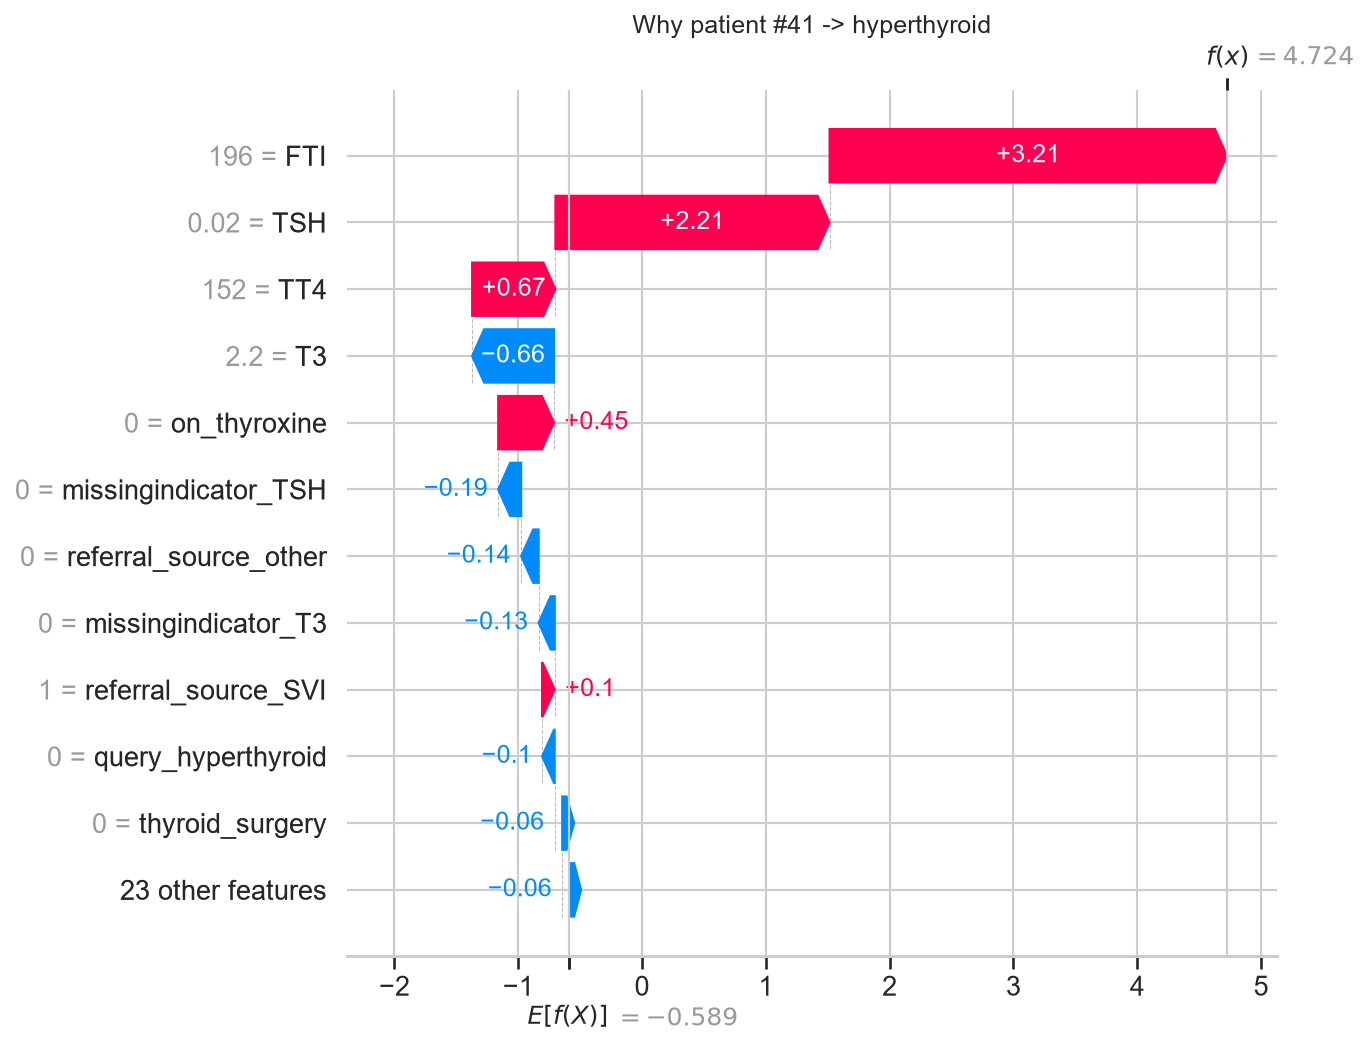
\includegraphics[width=0.97\columnwidth]{thyroid_waterfall_hyper.png}
\caption{Per-prediction SHAP waterfall: hyperthyroid. FTI and suppressed TSH
dominate.}
\label{fig:wf_hyper}
\end{figure}

\begin{figure}[t]
\centering
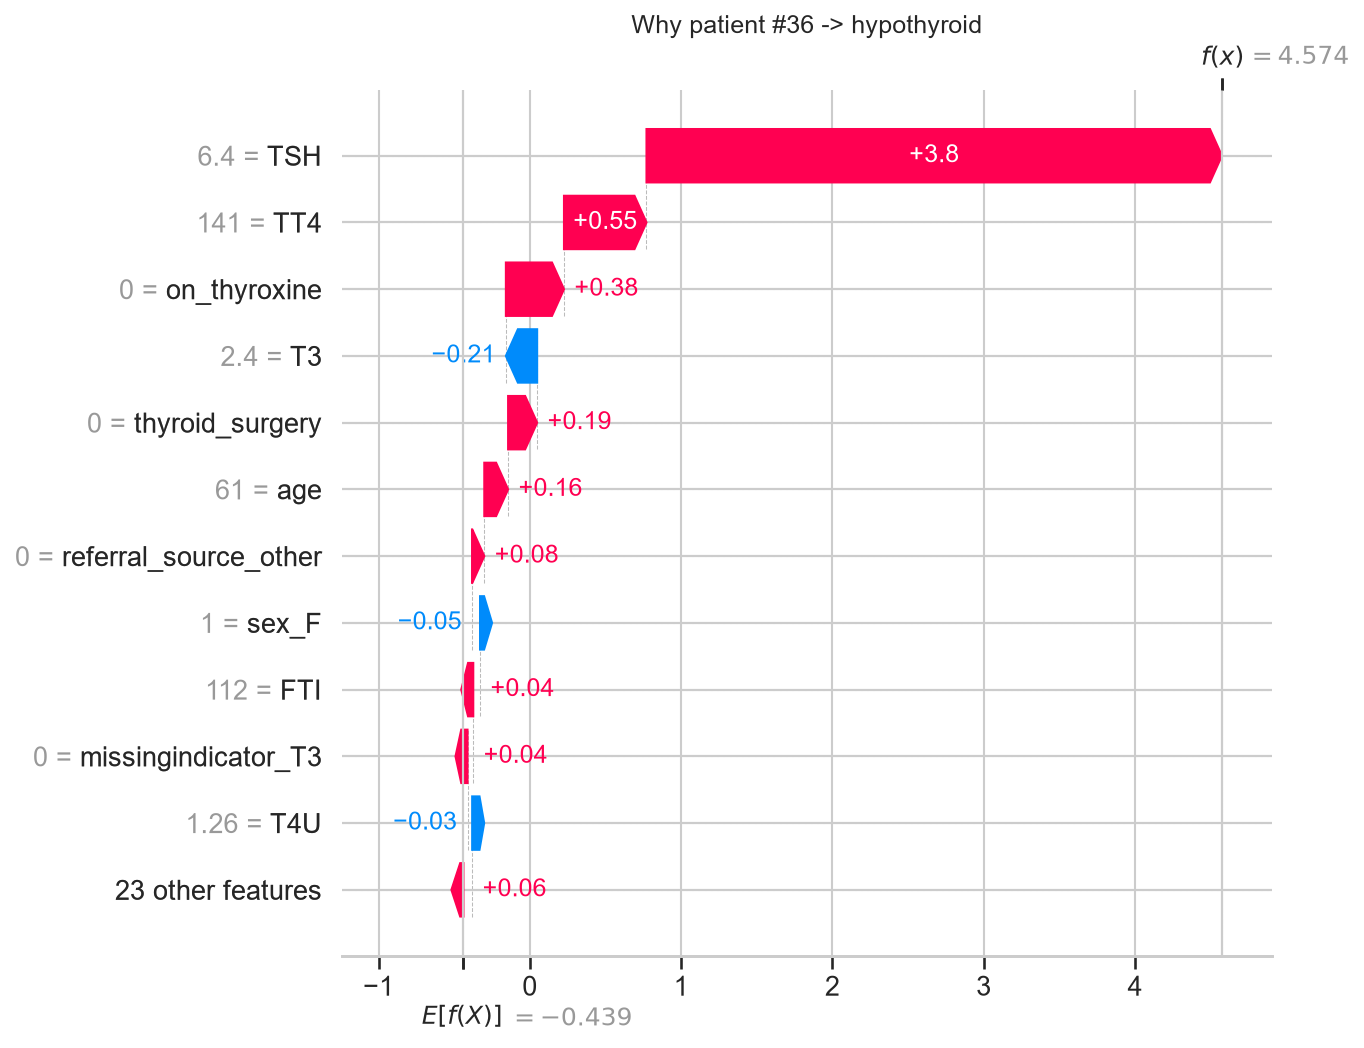
\includegraphics[width=0.97\columnwidth]{thyroid_waterfall_hypo.png}
\caption{Per-prediction SHAP waterfall: hypothyroid. Elevated TSH dominates.}
\label{fig:wf_hypo}
\end{figure}

\begin{figure}[t]
\centering
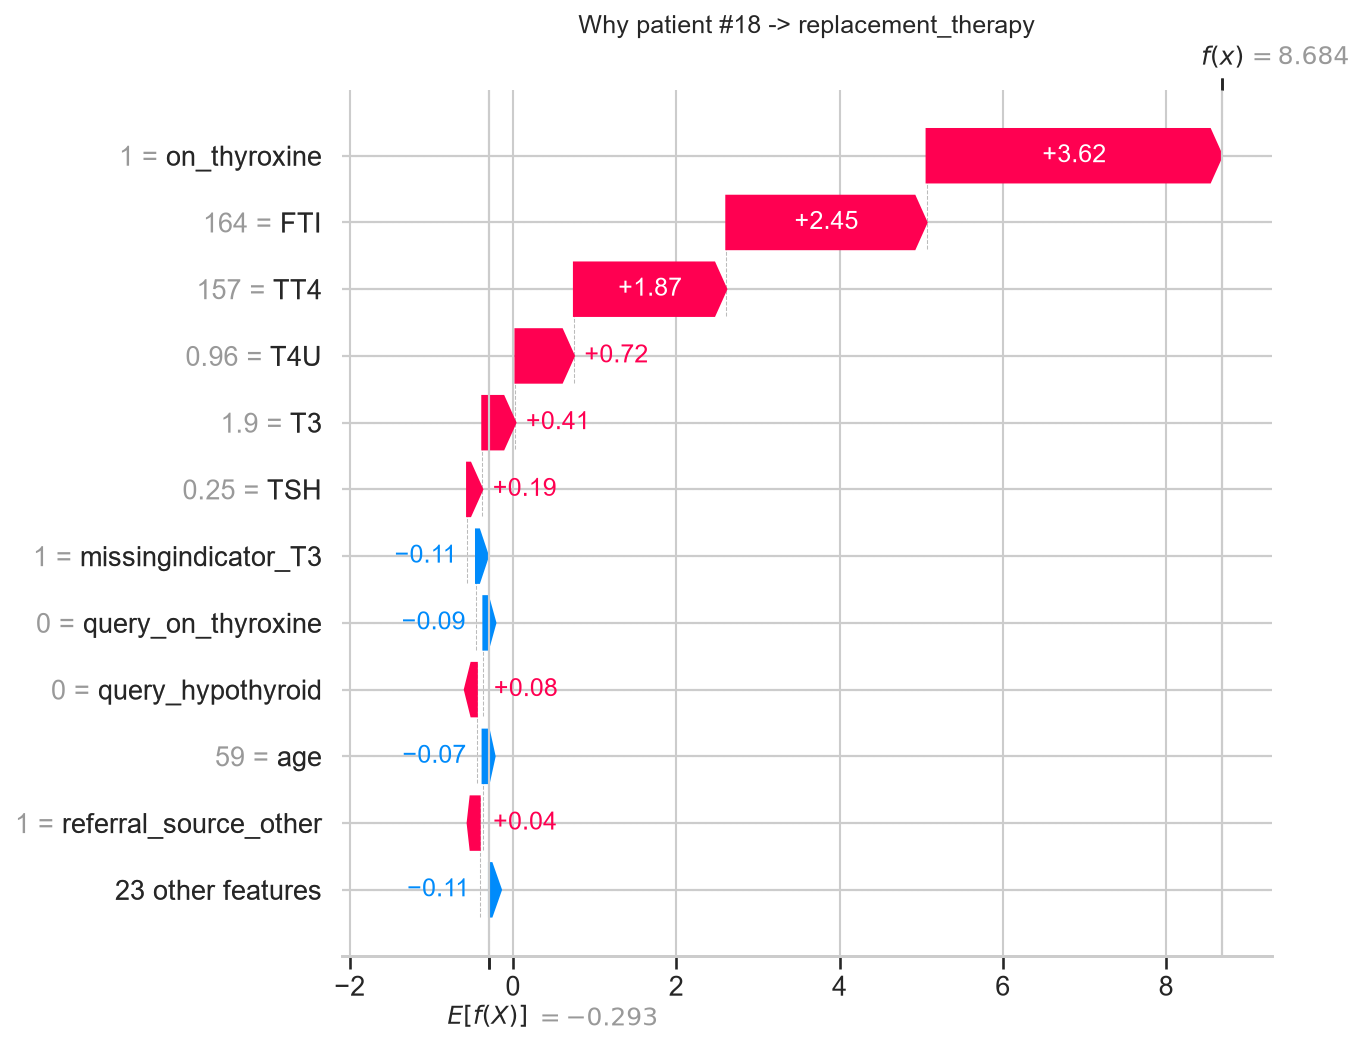
\includegraphics[width=0.97\columnwidth]{thyroid_waterfall_replace.png}
\caption{Per-prediction SHAP waterfall: replacement therapy. The
\textit{on\_thyroxine} history flag is decisive.}
\label{fig:wf_rep}
\end{figure}

\section{Discussion}
The study shows that a carefully trained tree-ensemble pipeline classifies seven
thyroid states with high accuracy and, more importantly, with reasoning that
matches physiology at the level of individual patients. The soft-voting hybrid is
the best of the classic trio and---unlike in smaller studies---its advantage over
the Random-Forest baseline is statistically significant, an effect attributable to
sample size rather than to a fundamentally different model. The principal
difficulty is the discordant-results class, where the model is appropriately
uncertain; this is a feature, not a bug, of an honest evaluation. The treatment of
informative missingness via indicator features, surfaced as genuinely predictive by
SHAP, is a practical lesson for laboratory-based ML.

\section{Limitations}
The archive is single-institution and decades old; external multi-centre
validation is required before clinical use. The seven-class grouping merges
fine-grained diagnoses and folds antithyroid-treatment codes into hyperthyroid.
Hyperparameters were only lightly tuned. SHAP attributions are associational, not
causal. Rare classes remain under-represented, limiting the reliability of their
per-class estimates.

\section{Conclusion}
We presented a detailed, reproducible, and explainable framework for seven-class
thyroid-disease classification, with an in-depth account of five tree-ensemble
models and exactly how they are trained, an imbalance-aware and leakage-safe
methodology, a statistically grounded comparison, and exact per-prediction SHAP
explanations that recover thyroid physiology. The hybrid achieves accuracy $0.945$
and macro-F1 $0.863$, with a significant improvement over the baseline. Future work
includes external validation, cost-sensitive learning for rare classes, SHAP
interaction analysis, and probability calibration for actionable confidence.

\begin{thebibliography}{1}
\bibitem{ref_garavan}
J.~R. Quinlan \emph{et al.}, ``Thyroid Disease Records,'' Garavan Institute, UCI
Machine Learning Repository, 1987.
\bibitem{ref_rf}
L.~Breiman, ``Random Forests,'' \emph{Machine Learning}, vol.~45, no.~1,
pp.~5--32, 2001.
\bibitem{ref_xgb}
T.~Chen and C.~Guestrin, ``XGBoost: A Scalable Tree Boosting System,'' in
\emph{Proc.\ ACM SIGKDD}, 2016, pp.~785--794.
\bibitem{ref_lightgbm}
G.~Ke \emph{et al.}, ``LightGBM: A Highly Efficient Gradient Boosting Decision
Tree,'' in \emph{NeurIPS}, 2017.
\bibitem{ref_stack}
D.~H. Wolpert, ``Stacked Generalization,'' \emph{Neural Networks}, vol.~5, no.~2,
pp.~241--259, 1992.
\bibitem{ref_shap}
S.~M. Lundberg and S.-I. Lee, ``A Unified Approach to Interpreting Model
Predictions,'' in \emph{NeurIPS}, 2017.
\bibitem{ref_treeshap}
S.~M. Lundberg \emph{et al.}, ``From Local Explanations to Global Understanding
with Explainable AI for Trees,'' \emph{Nat.\ Mach.\ Intell.}, vol.~2, pp.~56--67,
2020.
\end{thebibliography}

\end{document}
